\documentclass{beamer}
%[aspectratio=169]   \usepackage[czech]{babel}
\usepackage{apo-lecture}
\usepackage{pdfpages}
\usepackage{pdfcomment}
\usepackage{listings}
\usepackage{array,multirow}

\subtitle{Lekce 06. Superskalární arichitektura\\a\\prediktory skoků}
\author{Pavel Píša \phantom{xxxxxxx} Petr Štěpán \\ \small\texttt{pisa@fel.cvut.cz}\phantom{xxxx}\small\texttt{stepan@fel.cvut.cz}}
\begin{document}

\maketitle

\section{Superscalární architektura}

\begin{frame}
\frametitle{Cíl dnešní přednášky}

\begin{itemize}
 \item Podívat se na další možné zrychlení procesoru, které navazuje na pipelining
 \item Predikce skoků jako velmi důležitá vlastnost superskalárních procesorů
 \item Obě tyto techniky se využívají jak v RISC-V procesorech, tak i ve všech současných procesorech
\end{itemize}

\end{frame}

\begin{frame}

\frametitle{Procesor s pipeline (z přednášky 5)}

Jak moc je složitá Hazard Unit?
\begin{columns}
\begin{column}{0.7\textwidth}
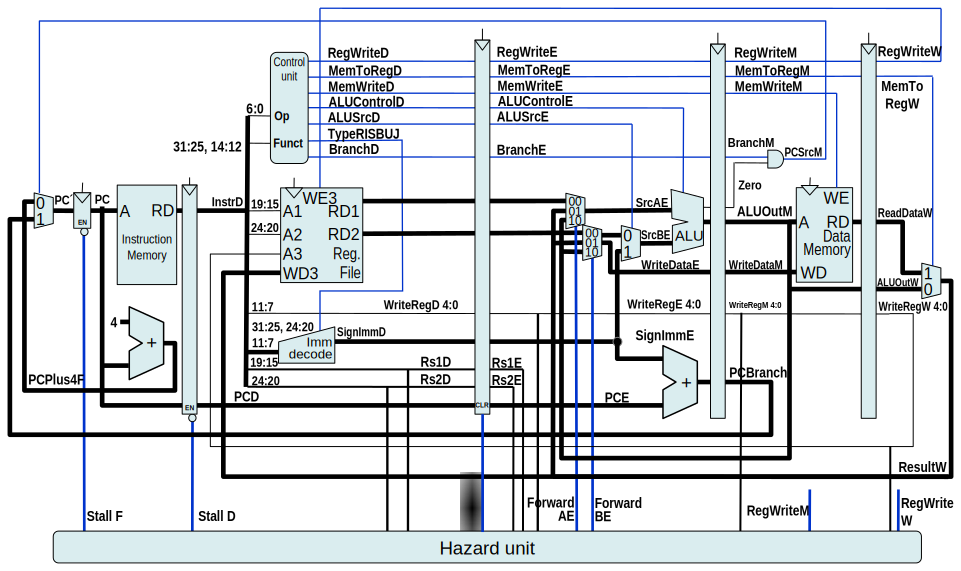
\includegraphics[width=\textwidth]{cpu_final_design.pdf}
\end{column}
\begin{column}{0.3\textwidth}
\tiny
\begin{itemize}
\item Pokud je RegWriteM==1, MemToRegM==0 a WriteRegM==RsE1 nebo RsE2 pak nastav ForwardAE na 2 nebo ForwardBE na 2
\item Pokud je RegWriteW==1, MemToRegW==0 a WriteRegW==RsE1 nebo RsE2 pak nastav ForwardAE na 1 nebo ForwardBE na 1
\item Pokud MemToRegM==1 a WriteRegW==Rs1E nebo Rs2E pak nastav pozastavení - STALL
\end{itemize}
\end{column}
\end{columns}
\end{frame}

\begin{frame}
\frametitle{Paralelismus na úrovni instrukcí}

Paralelní zpracování na úrovni instrukcí (Instruction Level Parallelism, ILP)
\begin{itemize}
 \item Pipelining -- paralelně se zpracovávají různé fáze různých instrukcí
 \item Superskalární procesor -- paralelně se zpracovávají stejné fáze různých instrukcí
\begin{itemize}
\item můžeme mít více jednotek ALU a provádět paralelně fáze EX více různých instrukcí
\item ve fázi fetch můžeme paralelně načítat více instrukcí jdoucích po sobě, tedy instrukci z adresy PC, PC+4, PC+8 a PC+12
\item jednotlivé fáze instrukcí jsou navíc zřetězené, takže po paralelním načtení 4 intrukcí, rovnou načítáme další 4 instrukce 
\end{itemize}
\end{itemize}

\end{frame}

\begin{frame}
\frametitle{Paralelismus na úrovni instrukcí}

Zřetězený procesor -- piplened procesor
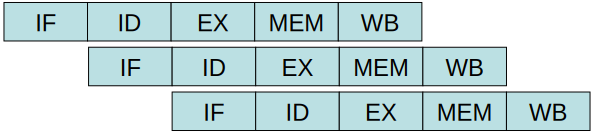
\includegraphics[width=0.85\textwidth]{pipeline.pdf}

Superskalární procesor -- super scalar procesor
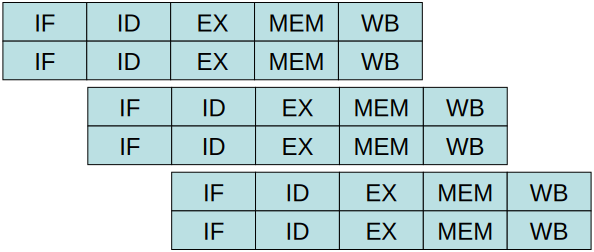
\includegraphics[width=0.85\textwidth]{superscalar.pdf}

\end{frame}

\begin{frame}
\frametitle{Superskalární procesory}

\begin{itemize}
\item mají IPC (Instruction Per Clock) větší než 1. 
  \begin{itemize}
  \item Normální i pipelined procesor mají neustále IPC=1
  \end{itemize}
\item Počet paralelních větví se nazývá šířka zřetězení (instruction pipeline width)
\item Existují dvě základní varianty:
  \begin{itemize}
  \item \textbf{Statická} superskalární architektura -- paralelně mohou být spuštěny jen instrukce jdoucí v programu za sebou.
    \begin{itemize}
    \item Pokud na sobě instrukce závisí vede to k pozastavení procesoru (stall).
    \end{itemize}
  \item \textbf{Dynamická} superskalární architektura -- paralelně mohou být spuštěny libovolné instrukce, které jsou přiravené k vykonávání. 
    \begin{itemize}
    \item Umožňuje předbíhání instrukcí tzv. out-of-order execution.
    \item Lépe využívá HW prostředky procesoru.
    \end{itemize}
  \end{itemize}
\end{itemize}

\end{frame}

\begin{frame}
\frametitle{Superskalární procesory}

\begin{itemize}
\item Jednotlivé paralelní větve mohou být \textbf{unifikované} -- tedy všechny větve jsou stejné a mohou provádět všechny typy operací
  \begin{itemize}
  \item V praxi by to byl zbytečně složitý procesor -- nepoužívá se
  \end{itemize}
\item Jednotlivé paralelní větve jsou \textbf{specializované} -- každá větev umí jen některé instrukce:
  \begin{itemize}
  \item instrukce pracující pouze s registry -- výpočty, porovnání
  \item instrukce pracující s pamětí -- načítání/ukládání dat z/do paměti
  \item instrukce skoku -- instrukce měnící PC
  \end{itemize}
\end{itemize}
\end{frame}


\begin{frame}
\frametitle{Superskalární architektura}
\begin{columns}
\begin{column}{0.55\textwidth}
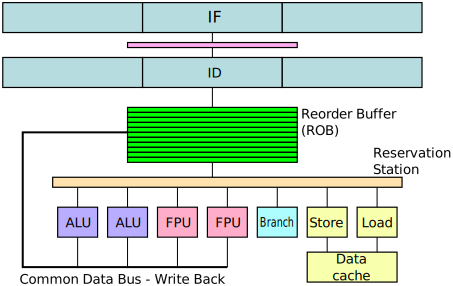
\includegraphics[width=\textwidth]{superscalar-architecture.pdf}
\end{column}
\begin{column}{0.45\textwidth}
\begin{itemize}
\item Základem architektury je reorder buffer, který pomocí přejměnování registrů umí zlepšit paralelizaci vykonávání instrukcí
\item Reservation Station rozšiřuje možnosti ukládání operandů pro operace a organizuje jejich vykonávání
\item Common Data Bus zajišťuje zapsání vypočtených hodnot do skutečných registrů i pro přejmenované registry.
\end{itemize}
\end{column}
\end{columns}
\end{frame}


\begin{frame}
\frametitle{Datové hazardy v superskalární architektůře}

\begin{itemize}
\item Příklad instrukcí a řešení přejmenováním
\end{itemize}
\end{frame}


\begin{frame}
\frametitle{Tomasulo algoritmus}

Robert Tomasulo z IBM vymyslel v roce 1967 algoritmus pro out-of-order vykonávání výpočtů na FPU.
V současné době je jeho modifikace základem architektury všech moderních procesorů.
\begin{itemize}
\item Zavedení instrukce do ROB a přejmenování registru výledku 
\item Zavedení instrukce do register station a čekání na připravená data
\item Provedení výpočtu a zapsání výsledku do přejmenovaného registru
\item Ukončení výpoštu nejstarší instrukce (kruhový buffer) z ROB a aktualizace systémového registru.
\end{itemize}
\end{frame}


\end{document}

